\begin{frame}{A lemezvándorlás és szubdukció felfedezése elmélete}
    Horváth Ferenc: Wegener-centeráium: Megszületett-e a kontinensvándorlás Newtonja? \cite{horvath}
    \vspace{10pt}
    
    \pause
    
    \begin{center}
    \begin{minipage}[c]{0.625\textwidth}
        \centering
        \fig{horvath_ferenc.png}
        
        Horváth Ferenc (1944.03.24.-2018.11.17.)
    \end{minipage}
    \end{center}
\end{frame}


\begin{frame}{Wegener elmélet}
    \begin{itemize}
        \item \textbf{Alfred Wegener} (1880-1930)
        \begin{itemize}
            \item 1912 január 6. német Földtani Társulat ülése, Farnkfurt: ``A földkéreg nagyformáinak (a kontinensek és az óceánok) alakulásageofizkai adatok alapján''
            \item 1912 január 10. Marburg: ``A kontinensek horizontális elmozdulása''
            \item 1912-ben két publikáció
            \item ``...a kontinesvándorlás Newtonja még nem született meg'' 1929
        \end{itemize}
    \end{itemize}
\end{frame}


\begin{frame}{Wegener modellje}
    \begin{center}
        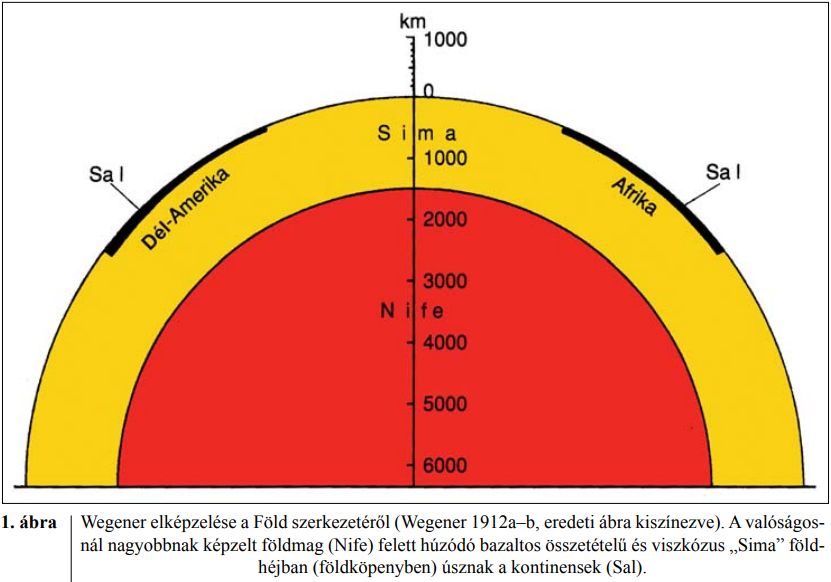
\includegraphics[width=0.525\textwidth]{wg_theory.png}
    \end{center}

    \begin{minipage}[c]{0.45\textwidth}
        \begin{itemize}
            \item kontinensek (Sal) belemerülnek és úsznak a földköpenyben (``Sima'')
            \item Sima vagy magma: bazaltos összetételű, viszkózus
            \item Nife: földmag
        \end{itemize}
    \end{minipage}
    \begin{minipage}[c]{0.45\textwidth}
    \begin{itemize}
        \item lehetséges hajtóerők
        \begin{itemize}
            \item Eötvös-erő (``Polflucht'')
            \item árapálysúrlódás
            \item köpenyáramlás
        \end{itemize}
    \end{itemize}
    \end{minipage}
\end{frame}


\begin{frame}{Lehetséges hajtóerők}
    \begin{figp}{\inc{wg_eotvos.png}}{}{0.47}{0.4}
        \begin{itemize}
            \item Eötvös Loránd fedezte fel (1905), $\ne$ Eötvös-effektus
            \item Föld- és potenciálfelületek alakja ellipszoid
            \item súlyerő vagy nehézségi erő (C) + ellenerő (T) $\rar$ egyenlítő felé mutató erő
        \end{itemize}
    \end{figp}
\end{frame}


\begin{frame}{Lehetséges hajtóerők}
    \begin{minipage}[c]{0.575\textwidth}
        \centering
        \inc{wg_tide.png}
    \end{minipage}
    \begin{minipage}[c]{0.35\textwidth}
        \begin{itemize}
            \item árapálymaximum $\ne$ Föld-Hold tömegközéppont egyenes
            \item Föld forgásának folyamatos lassítása, nyugati drift
            \item szilárd Föld, hidroszféra, atmoszféra nem tökéletesen rugalmas (viszkoelasztikus) $\rar$ 2-3$^\circ$ eltérés keletebbre
        \end{itemize}
    \end{minipage}
\end{frame}


\begin{frame}{Lehetséges hajtóerők}
    \begin{figp}{\inc{wg_cont_drift.png}}{Wegener elmélete a kontinensek vándorlásáról.}{0.45}{0.4}
        \begin{itemize}
            \item köpenyben radioaktív hőtermelés $\rar$ konvektív áramlás
            \item felfelé áramlás $\rar$ óceánközepi-hátság
            \item ütköző kontinensek $\rar$ lánchegységek
            \item lehetséges erőhatások nagyon kicsik $\rar$ ``sima'' teljesen viszkózus (folyadékszerű) viselkedés
            \item kis erők $\rar$ kis elmozdulások $\rar$ geológiai időskálákon, nagy elmozdulás
        \end{itemize}
    \end{figp}
\end{frame}


\begin{frame}{A kontinensvándorlás elmélet kritikusa}
    \begin{itemize}
        \item \textbf{Harold Jeffreys} (1891-1989); matematikus, csillagász, geofizikus; Naprendszer kialakulás, Föld belső szerkezet
        \item mag külső héja folyadékszerű (nincs nyíróhullám)
        \item Föld többi része szilárd, nyíróhullámok jelenléte $\rar$ minden erőhatás deformációval kompenzálódik
        \item Wegener féle erőhatások $\ll$ köpeny szakítási szilárdsága
        \item Jeffreys: A Földön minden hőmérséklet- és nyomáskülönbség már régen kiegyenlítődött
    \end{itemize}
\end{frame}


\begin{frame}{A Wegener elmélet támogatói - geológusok, fizikusok}
    \begin{itemize}
        \item \textbf{John Joly} (1857-1933); fizikus, természetes radioaktivitás;
        \item Kelvin földmodell (térben homogén paraméterek, konduktív hőterjedéssel hülő Föld), 96 (30) Ma $\leftrightarrow$ geológiai ismeretek
        \item együttműködés Rutherforddal, devon korú kőzetek korolása; 400 Ma (1913)
        \item nagytektonikai folyamatok energiája radioaktív hőtermelésből
        \item radioaktív elemek hőtermelése $\rar$ fokozatosan felhalmozódó hő $\rar$ ciklikus (100-200 Ma) bazaltömlés (ma ``forró folt'' vulkanizmus)
        \item bazaltos köpenyanyag áramlása a felszínre $\rar$ kontinesek vándorlása
    \end{itemize}
\end{frame}


\begin{frame}{A Wegener elmélet támogatói - geológusok, fizikusok}
    \begin{itemize}
        \item \textbf{Arthur Holmes} (1890-1965); geológus;
        \item radioaktív- és egyéb kormeghatározások $\rar$ Föld kora: 1600 Ma
        \item egyetértett Joly érvelésével
        \item ``...meggyőző bizonyítékaink vannak, amelyek a kontinesek egykori vándorlására mutatnak, mégpedig úgy, ahogy azt Wegener javasolta''
        \item Emile Argand (1879-1940): ``Mi nem szándékozunk a tektonikát visszavezetni a fizikára, ez a jövő feladata.''
    \end{itemize}
\end{frame}


\begin{frame}{A Wegener elmélet támogatói - geológusok, fizikusok}
    \begin{itemize}
        \item \textbf{Frank B. Taylor} (1860-1938); Harvard Egyetem tanulmányok: geológia, asztronómia; Amerikai Földtani Szolgálat (USGS) glaciológiai osztálya;
        \item kontinesek egyenlítő felé mozgása $\rar$ alpi-himalája-melanéziai és cirkum-pacifikus hegységrendszer kialakulására (1910)
        \item Eötvös-erő hatása? megfelelően nagy?
    \end{itemize}
    
    \begin{itemize}
        \item \textbf{W. Lambert} (1879-1968); USGS, geodéta;
        \item Eötvös-erő nagyságának kiszámítása: 30$^\circ$ északi szélességen 1 km átmérőjű kéregsűrűségű gömb
        \item súrlódásmentes gördülés 4-5 m/s átlagsebesség
        \item ha köpeny anyag folyadékszerű $\rar$ geológiai időskálán ezer km-es mozgások
    \end{itemize}
\end{frame}


\begin{frame}{A Wegener elmélet támogatói}
    \begin{minic}{0.95}
        \centering
        \inc{wg_taylor_theory.png}
    \end{minic}
\end{frame}


\begin{frame}{A Wegener elmélet támogatói - geológusok, fizikusok}
    \begin{itemize}
        \item \textbf{Reginald A. Daly} (1871-1957); tanulmányok: Torontói Egyetem, Harvard, Heidelberg, Párizs; MIT fizikai geológia; Harvard Egyetem: a geológia professzora;
        \item Lambert legfőbb támogatója; kontinesvándorlást hajtó mechanizmus keresése
        \item négy lehetséges hajtóerő
        \begin{itemize}
            \item árapálysúrlódás $\rar$ nyugati drift
            \item geoszinklinális mélyáramlások
            \item Eötvös-erő
            \item orogenezis során kialakuló feszültség
        \end{itemize}
        \item szerinte: egyik erő sem elegendő; többet kell tudni a földi anyagok reológiájáról
    \end{itemize}
\end{frame}

\begin{frame}{A Wegener elmélet támogatói - geológusok, fizikusok}
    \begin{itemize}
        \item \textit{Dél-Afrikai expedíció} Carnegie Intézet támogatásával Bushweld magmás komplexum (1922)
        \item Reginald A. Daly, F. Wright (1877-1953) petrológus, G. Molengraaf (1860-1942) delfti professzor, Alexander du Toit (1878-1948) geológus;
        \item Daly és Wright meggyőzése a kontinensvándorlás elmélet helyességéről; ``lobbizás'' $\rar$ Carnegie Intézet anyagi támogatása du Toit Dél-Amerika, Karoo Formáció feltárása
        \item adatok feldolgozása $\rar$ Dél-Afrika és Dél-Amerika karbon-jura képződményei, rétegtani, őslénytani, kőzettani hasonlóságok $\rar$ két kontinens karbontól összetartozott, középső jura szétszakadás
        \item bizonyíték a kontinesvándorlásra
    \end{itemize}
\end{frame}


\begin{frame}{A Wegener elmélet bizonyítékai}
    \begin{minipage}[c]{0.525\textwidth}
        \inc{wg_daly_theory.png}
    \end{minipage}
    \begin{minipage}[c]{0.45\textwidth}
        \begin{itemize}
            \item geoszinklinálisokban folyamatosan felhalmozódó üledék $\rar$ kéreg betüremkedik a folyadékszerű bazaltba (``glassy basalt'')
            
        \end{itemize}
    \end{minipage}
    \begin{itemize}
        \item bazalt peremek felé mozog $\rar$ peremek emelkednek $\rar$ üledék behordása
        \item mélyebbre süllyedő kéreg felmelegedik $\rar$ gyökér destabilizálódik, kiszakad, lesüllyed
        \item szabad térbe benyomul az emelt kéregrész $\rar$ üledéket felgyűri $\rar$ hegységképződés
    \end{itemize}
\end{frame}


\begin{frame}{A Wegener elmélet bizonyítékai}
    \begin{itemize}
        \item \textbf{William Bowie} (1872-1940), USGS geodéziai osztály vezetője;
        \item ``... a világ csillagászai és geodétái elhatározták, hogy pontos tesztmérésekkel ellenőrzik Wegener hipotézisét'' (New York Times, 1925)
        \item világméretű háromszögelés hálózat, rádiohullámok futási ideje $\rar$ kontinensek elmozdulása
        \item hibaszámítások: pontosság néhány m/év sebesség kimutatására nem elegendő (Oroskes 1999)
    \end{itemize}
\end{frame}


\begin{frame}{A Wegener elmélet bizonyítékai}
    \begin{itemize}
        \item \textbf{Felix Vening Meinesz} (1887-1966); holland mérnök, nemzeti geodéziai szolgálat; tengeri gravitációs mérések
        \item speciális kettős inga kifejlesztése, enyhén ingatag talapzaton is működőképes
        \item holland haditengerészet tengeralattjárója (1923-1927); több száz tenger alatti mérés
        \item mélytengeri Jáva-árok: -120, -140 mgal anomális (kontinentális terület, izosztatikus kompenzáció miatt $\pm$ 10-30 mgal)
        \item mélytengeri árok mentén kompressziós kéregbetüremkedés
        \item Carnegie Intézet, tengeralattjáró: Karib-árok mentén méresek (1932-1937); hasonló negatív gravitációs anomália
        \item mérésekben részt vettek: \textbf{Harry Hess} (1906-1969), \textbf{Maurice Ewing} (1906-1974) II.vh alatt mérések, 60-as években lemeztektonika megszületésénél fontos szerep
    \end{itemize}
\end{frame}


\begin{frame}{A lemeztektonikától napjainkig}
    \begin{itemize}
        \item Harry Hess gravitációs mérések $\rar$ árkoknál betüremkedő réteg modellje $\rar$ óceáni kéreg és a köpeny is mozog, ütközik és gyűrődik
        \item Harry Hess: ócáni aljzat szétterülésének elmélete (ocean-floor spreading) (1962)
        \item kontinensek litoszférán utazó, óceáni területekhez kapcsolódó lemezek részei, amelyek a részlegesen olvadt aztenoszférán mozognak
        \item megszületett a lemeztektonika elmélete
    \end{itemize}
\end{frame}


\begin{frame}{A lemezmozgás dinamikája}
    \begin{minic}{0.68}
        \centering
        \inc{wg_slab_mechanics.png}
    \end{minic}
    $F_{\text{SU}}$, $F_{\text{SP}}$: ``árokszívás'', indukált köpenyáramlás húzó hatása; $R_{\text{R}}$: lemez és asztenoszféra - súrlódás; $R_{\text{B}}$ alátolódó lemez hajlításához szükséges feszültség; $R_{\text{S}}$ felső köpenyben, mélységgel növekvő viszkozitás, sűrlódási ellenállás; $R_{\text{O}}$ kontinentális- és alátolódó lemez - súrlódás; $R_{\text{DO}}$, $R_{\text{DC}}$: óceáni- és kontinetális lemez, asztenoszféra köpenyáramlás súrlódás
\end{frame}


\begin{frame}{A lemezmozgás dinamikája}
    \begin{center}
        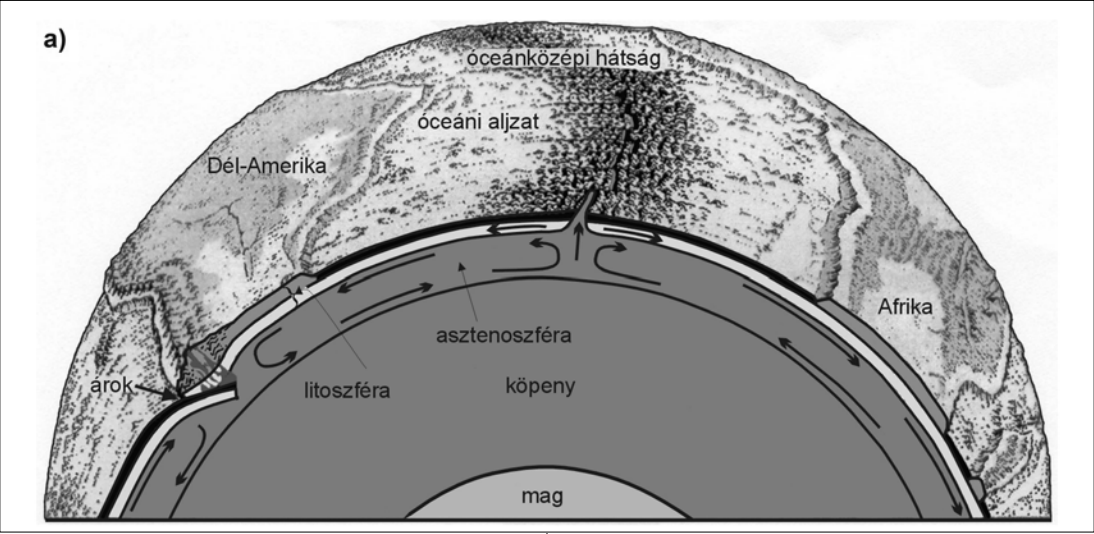
\includegraphics[width=0.85\textwidth]{wg_cell_flow.png}
    \end{center}
    \begin{itemize}
        \item lemeztektonika kezdeti időszakáig a köpenyáramlást tekintették a legfőbb mozgatóerőnek
        \item cellaszerű áramlás
        \item feláramlás: hátságoknál lemezek távolítása; leáramlás: lemezeket lefelé húzza
    \end{itemize}
\end{frame}


\begin{frame}{A lemezmozgás dinamikája}
    \begin{center}
        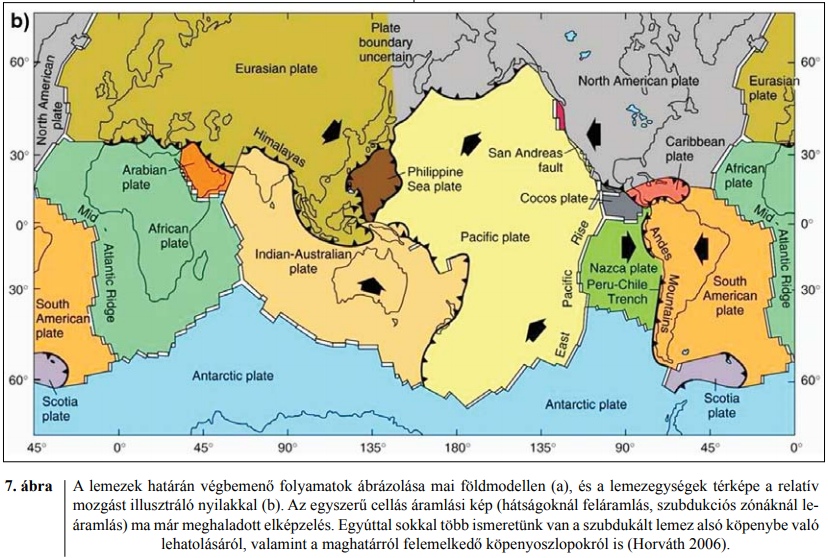
\includegraphics[width=0.95\textwidth]{wg_global_plate_movement.png}
    \end{center}
\end{frame}


\begin{frame}{A lemezmozgás dinamikája}
    \begin{itemize}
        \item hátságok mélytengeri árkok bonyolult geometria $\rar$ szabálytalan áramlási cella geometria
        \item hátságok helyzete nem fix, mélytengeri árkokhoz képest változó
        \item Antarktiszi-lemez növekedik, hátságok magukat tólják el az Antarktisztól?
        \item Kelet-Pacifikus-hátság Kalifornia déli részénél eltűnik; 30 Ma ezelőtt 1000 km-el nyugatabbra helyezkedett el
        \item hátságok központi hasadékvölgye = szakadási vonal a litoszférában, lemezekkel együtt mozog; asztenoszféra anyagának felszínre törése
    \end{itemize}
\end{frame}


\begin{frame}{A lemezek mozgásának abszolút sebessége}
    Forsyth és Uyeda (1975); köpeny hőoszlopok (mantle plumes) és forró folt (hot spot) mint abszolút koordinátarendszer fix pontjai
    
    \begin{center}
        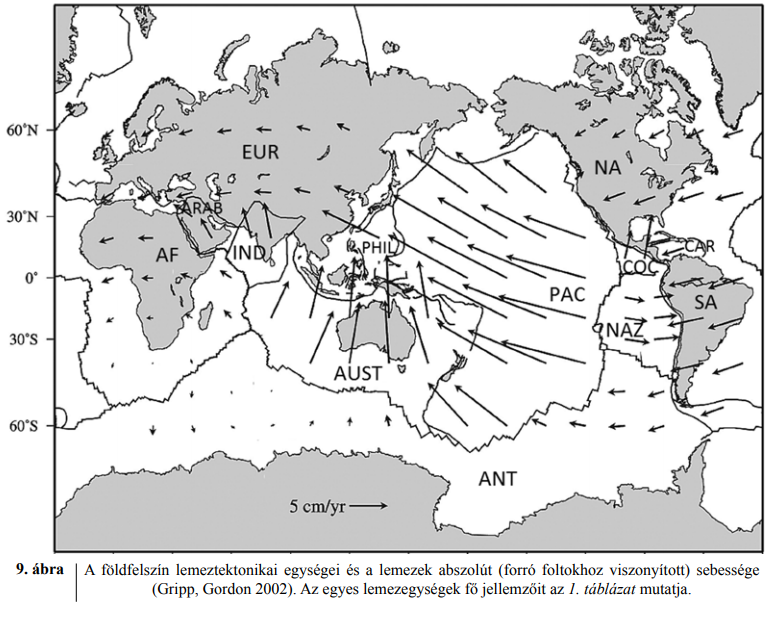
\includegraphics[width=0.75\textwidth]{wg_rel_vel_hotspot.png}
    \end{center}
\end{frame}


\begin{frame}{A lemezek mozgásának abszolút sebessége}
    \begin{center}
        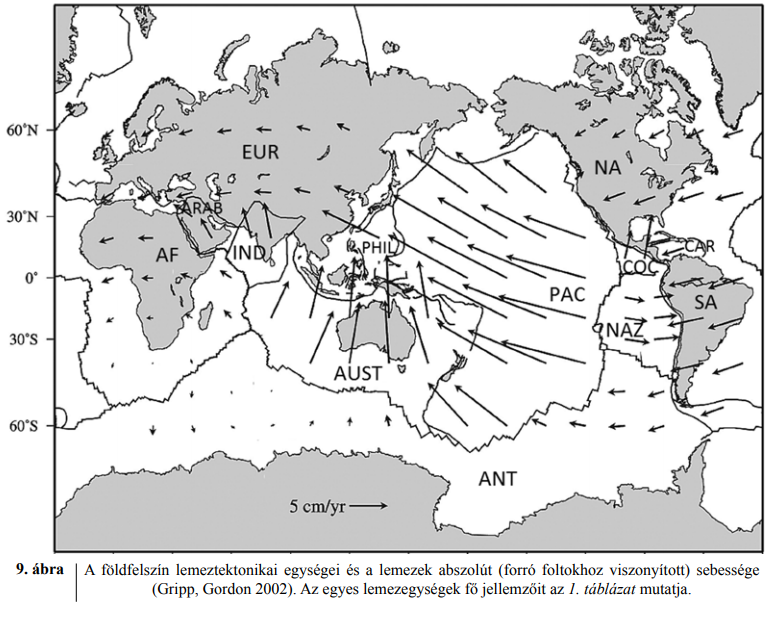
\includegraphics[width=0.675\textwidth]{wg_rel_vel_hotspot.png}
    \end{center}
    Pacifikus-lemez, teljes litoszféra rendszer mozgási energiájának 2/3-a; Pacifikus-, Indiai-Ausztrál- és Nazca-lemez a teljes energia 95\%
\end{frame}


\begin{frame}{A lemezek mozgásának abszolút sebessége}
    \begin{center}
        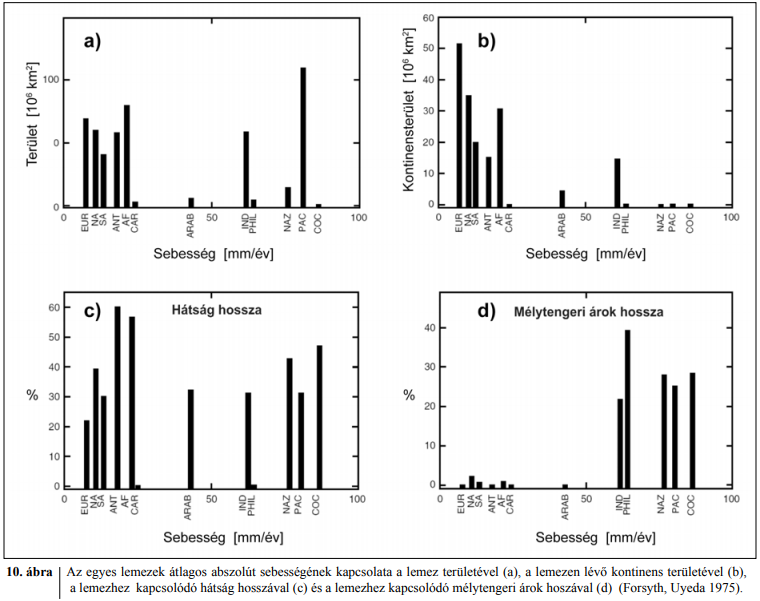
\includegraphics[width=0.7\textwidth]{wg_slab_vel_corr.png}
    \end{center}
    \begin{itemize}
        \item nincs korreláció a sebességgel: lemezméret és hátsághossz
        \item korreláció a sebességgel: kontinesterület és mélytengeri árok hossza
    \end{itemize}
\end{frame}


\begin{frame}{Új földmodell a szeizmikus tomográfia alapján}
    \begin{center}
        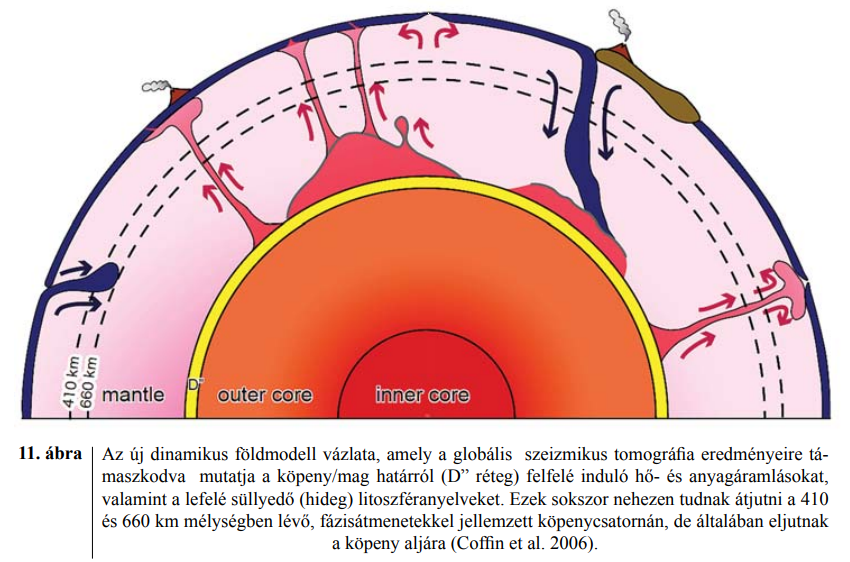
\includegraphics[width=0.7\textwidth]{wg_theory_today.png}
    \end{center}
    \begin{itemize}
        \item bazaltömlések a D'' hőáramlási oszlopokhoz kapcsolódnak
        \item leáramlások a szubdukált lemezekhez, D'' rétege érkeznek
        \item mai elképzelés szerint ez a két fő teljes köpenyre kiterjedő áramlástípus mozgatja a lemezeket
    \end{itemize}
\end{frame}
